\documentclass[10pt]{article}
\usepackage[utf8]{inputenc}
\usepackage[T1]{fontenc}
\usepackage{amsmath}
\usepackage{amsfonts}
\usepackage{amssymb}
\usepackage[version=4]{mhchem}
\usepackage{stmaryrd}
\usepackage{graphicx}
\usepackage[export]{adjustbox}
\graphicspath{ {./images/} }

\DeclareUnicodeCharacter{21D2}{\ifmmode\Rightarrow\else{$\Rightarrow$}\fi}

\begin{document}
Last line we have established that the sequence $\left\{k_{t+1}\right\}_{t=0}^{\infty}$ solves the (SP) problem

$$
=F\left(k_{+}, k_{++1}\right) \text { (denone) }
$$

(SP)

$$
\begin{aligned}
& \left.\operatorname{Max}_{\left\{k_{+1}\right\}_{+=0}^{\infty}} \sum_{t=0}^{\infty} p^{+} u\left(f \mid k_{+}\right)-k_{++1}\right) \\
& \text { s.t. } \underbrace{0 \leq k_{++1} \leq f\left(k_{+}\right)}_{k_{0} \text { isgiven }}, t=1,2, \ldots \\
& k_{++1} \in \Gamma\left(k_{+}\right) \text {(denote) }
\end{aligned}
$$

if and only if it solves

$$
\begin{gathered}
\left(E(E): \begin{array}{cc}
u^{\prime}\left(f\left(k_{t}\right)-k_{t+1}\right)= & \beta f^{\prime}\left(k_{t+1}\right) u^{\prime}\left(f\left(k_{t+1}\right)-k_{t+2}\right) \\
k_{0} \text { given } & t=1,2, \ldots
\end{array}\right.
\end{gathered}
$$

and

$$
\text { (TC) } \lim _{x \rightarrow \infty} \beta^{+} u^{\prime}\left(f\left(k_{+}\right)-k_{+1}\right) \cdot f^{\prime}\left(k_{+}\right) \cdot k_{+}=0
$$

$\Rightarrow(S P)$ san be solved by finding a sequence $\{k+1\}$ that solves (EE) (e.g. "guess and verify" or lim. to a finite horzon probl.) and then verifying that (TC) is satisfiled.

Solving the infinite horizon OGM\\
General strategy: sind a solution of the (EE)

\begin{itemize}
  \item check that (TC) is satisfied
\end{itemize}

What's a good "candidate" solution?\\
Example 1: The limit solution of the finite horizon model Recall from lost class:

$$
\begin{aligned}
& u(c)=\log (c), \quad f(k)=k k \Rightarrow \\
& \Rightarrow S_{4}=\beta \cdot \frac{1-\beta^{T-t}}{1-\beta^{T-t+1}} \rightarrow \beta \quad \text { as } T \rightarrow \infty
\end{aligned}
$$

⇒ Let's try $k_{++1}=\beta R k_{+}$as a possible solution\\
(EE): $\frac{1}{R k_{+}-\beta R k_{+}}=\beta R \frac{1}{R k_{++1}-\beta R k_{++1}}$

$$
k_{++1}=\beta R k_{+} \text {- indeed holds }
$$

(TC): $\lim _{t \rightarrow \infty} \beta^{t} R \cdot \frac{1}{R k_{+}-\beta k k_{+}} \cdot k_{+}=\lim _{t \rightarrow \infty} \beta^{t} \cdot \frac{1}{1-\beta}=0$ algo holds ⇒\\
$\Rightarrow k_{+1}=\beta R k_{+}$is the optimal poth!\\
Example 2: We can try to greess the frundional form of the solution by looking at the (EE):

$$
u(c)=\log (c), \quad f(k)=A k^{\alpha}
$$

(EE): $\frac{1}{A k_{+}^{\alpha}-k_{++1}}=\beta A \alpha k_{++1}^{\alpha-1} \cdot \frac{1}{A k_{+1}^{\alpha}-k_{++2}}$\\
Guess: $k_{++1}=S_{+} \cdot A k_{+}^{\alpha}$\\
i.e. guess that the samigs rate is constant

$$
\begin{aligned}
& \frac{1}{(1-s) A_{1} k_{+}^{\alpha}}=\beta \alpha \frac{A k_{+++}^{\alpha}}{k_{++1}} \cdot \frac{1}{k_{+-1} \text { SHk } k_{++\alpha}^{\alpha}} \\
& k_{++1}-n 1
\end{aligned}
$$

$$
\begin{aligned}
& \frac{k_{++1}}{A k_{+} \alpha}=\beta \alpha \\
& =s \\
& =s \text { (by guess) }
\end{aligned} \Rightarrow s=\beta \alpha
$$

Check the (TC):

$$
\begin{aligned}
& \lim _{t \rightarrow \infty} \beta^{+} A \alpha k_{+}^{\alpha-1} \cdot \frac{1}{(1-s) A k_{+}^{\alpha}} \cdot k_{+}= \\
& =\lim _{t \rightarrow \infty} \beta^{+} A \alpha \frac{k_{+}^{\alpha}}{(1-s) A k_{+}^{\alpha}}=0 \quad \text { holds! } \\
& \Rightarrow k_{++1}=\beta \cdot \alpha \cdot A k_{+}^{\alpha}, t \geq 0 \quad \text { is the optimal } \\
& k_{0} \text { given }
\end{aligned}
$$

This approach is called "Guess and verify."\\
Intuition: $\beta^{T} \Rightarrow$ more partient, value future consumption more ⇒\\
⇒ invest more\\
Some properties of this solution:\\
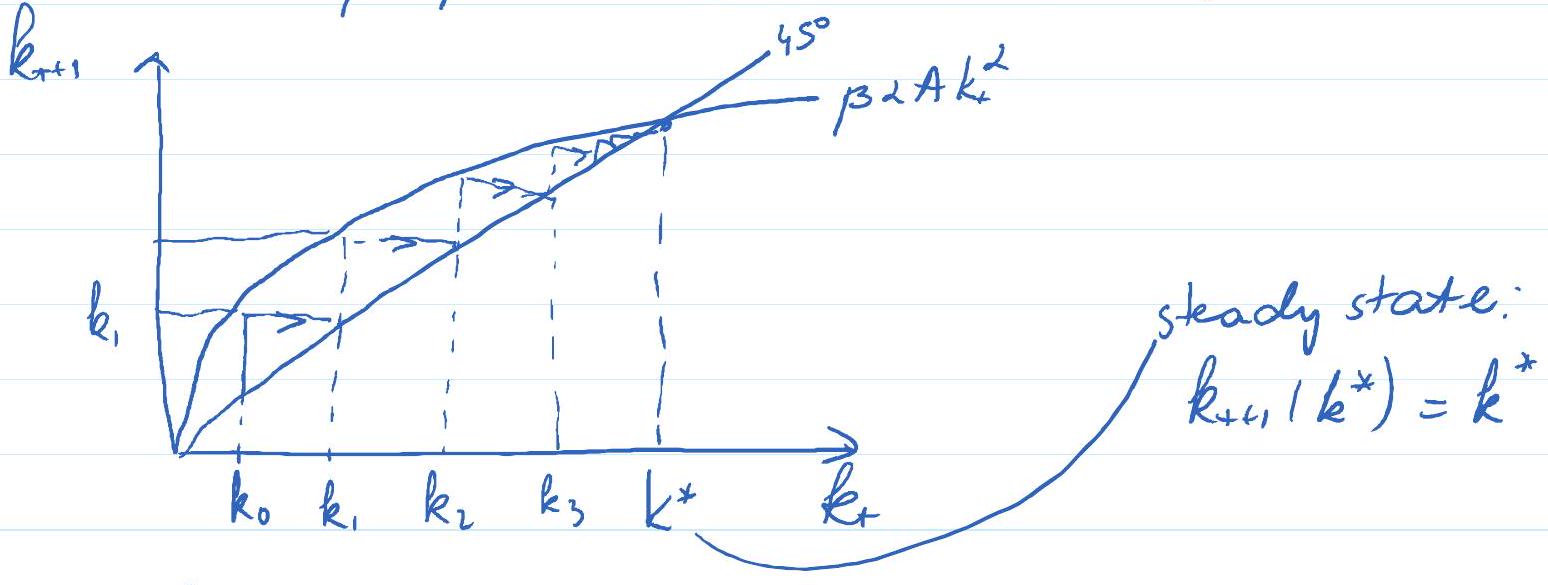
\includegraphics[max width=\textwidth, alt={}, center]{f4cb1c48-88bb-421e-95a2-79ed08ccdae7-3_585_1548_1654_177}\\
$k_{t} \rightarrow k^{*}, t \rightarrow \infty$

Steady State\\
Somettimes we are interested only in finding the steady-state (analyzing long-run effects of changes in economic environments).

Steady state: all variables are constant over time.

$$
\left(k_{+}=k^{*}, \quad \forall t\right)
$$

This is easy:

\begin{enumerate}
  \item Tust solve the (EE):
\end{enumerate}

$$
\begin{aligned}
& u^{\prime}\left(f\left(k^{*}\right)-k^{*}\right)=\beta f^{\prime}\left(k^{*}\right) \cdot u^{\prime}\left(f\left(k^{*}\right)-k^{*}\right) \\
& \Rightarrow \beta f^{\prime}\left(k^{*}\right)=1
\end{aligned}
$$

(In the steady state the marginal product of capital $\left.f^{\prime}\left(k^{*}\right)=\frac{1}{\beta}\right)$\\
2) (TC) holds by default:

$$
\lim _{T \rightarrow \infty} \beta^{T} \underbrace{\left.f^{\prime}\left(k^{*}\right) \cdot u^{\prime}\left(f \mid k^{*}\right)-k^{*}\right) \cdot k^{*}}_{\text {const }}=0
$$

Therefore, any path $\left\{k_{4}\right\}_{+=0}^{\infty}$ that converges to the steady state satisfies (TC)

The question though is whether (under which conditions) $\left\{k_{+1}\right\}_{+=0}^{\infty}$ converges to a steady statt...

\section*{Open questions}
Thus, we know

\begin{itemize}
  \item how to find the Strady State in the optimal growth
  \item how to solve it analytically for some $U(I) \& f 1$.$) .$
\end{itemize}

But what if analytral solution does not exist?

\begin{itemize}
  \item We could still try to find the steady state numericaly
  \item Use the numerical methods to find the path of convergence to the steady state (if the economy converges to a steady stake from $k_{0}$ )...
\end{itemize}

Can we do more? Iestablish analytical properties of $\left(k_{t+1}\right)_{t=0}^{\infty}$ ?\\
statility of the steady state.'\\
New tools needed....

It turns out that a lot more can be achieved if we reformulate (SP) recursively and use Dynamic Programming Theory to characterize the solution!

Dynamic Programming\\
Denote by $V\left(k_{0}\right)$ the indivect usility function obtained after (SP) is solved:\\
(*) $\quad V\left(k_{0}\right)=\max _{\left\{k_{++1}\right\}=0}^{\infty}\left\{\sum_{t=0}^{\infty} \beta^{t} F\left(k_{t}, k_{t+1}\right) \mid\right.$ s.t. $\begin{array}{l}k_{++1} \in \Gamma\left(k_{1}\right), t=0,1, \ldots \\ k_{0} \text { is isiven }\end{array}$\\
Since $\max _{x, y} f(x, y)=\max _{x}\left\{\max _{y} f(x, y)\right\}$, we can vewrite ( $*$ ) as:

$$
\begin{aligned}
& V\left(k_{0}\right)=\max _{k_{1}}\left\{\max _{\left\{k_{2}, k_{3}, \ldots\right\}}\left\{\sum_{t=0}^{\infty} \beta^{+} F\left(k_{+}, k_{++1}\right) \mid s . t . k_{k_{1} \in \Gamma} \in \Gamma\left(k_{1}\right), t=1,2, \cdots\right\} \mid\right. \\
& \text { s.t. } k_{1} \in T\left(k_{0}\right) \text {, koisgiven? } \\
& =f\left(k_{0}, k_{1}\right)+\beta \cdot \sum_{t=0}^{\infty} \beta^{+} F\left(k_{t+1}, k_{++2}\right) \\
& \text { does not depend } x_{0}^{t=0}\left\{k_{2} k_{3}, \ldots\right\} \text {. }=V\left(k_{1}\right)!!!
\end{aligned}
$$

$$
\begin{aligned}
& \text { s.t. } k_{1} \in\left[\left(k_{0}\right), k_{0} \text { is grean }\right]
\end{aligned}
$$

The original decision problem satisfies the\\
Principle of Optimality: given the chorce of $k_{1}$, the remaining $\left\{k_{2}, k_{3}, \ldots\right\}$ are also the outcone of the maximization problem (which is indepent of bo).

$$
V\left(k_{0}\right)=\max _{k_{1}}\left\{F\left(k_{0}, k_{1}\right)+\beta V\left(k_{1}\right)\right\}
$$

Here V ( $k_{0}$ ) - the value which the agent obtains it starts with koo and chooses $\left\{k_{1}, k_{2}, k_{3}, \ldots\right\}$

Here V ( $k_{0}$ ) - the value which the agent obtains it starts with ko and chooses $\left\{k_{1}, k_{2}, k_{3}, \ldots\right\}$.\\
$V\left(k_{1}\right)$ - the value - 11 - if starts with $k_{1}$ and chooses $\left\{k_{2}, k_{3}, k_{4} \cdot\right\}$.

Note: we could similarly rewrite

$$
V\left(k_{1}\right)=\max _{k_{2}}\left\{F\left(k_{1}, k_{2}\right)+\beta V\left(k_{2}\right)\right\}
$$

Or for period $t$ :

$$
V\left(k_{t}\right)=\max _{k_{t+1}}\left\{F\left(k_{t}, k_{t+1}\right)+\beta V\left(k_{t+1}\right)\right\}
$$

Intuitively, the agent makes an optimal decision in period $t$ knowing that he will behave optimally from period $t+1$ enward / and hence will get indivect utility $V\left(k_{+1}\right)$ )

In fact, we do not need the time index: tuink in terms of "today" and "tomorrow" only:\\
(p) $V(k)=\max _{k^{\prime}}\left\{F\left(k_{1} k^{\prime}\right)+\beta V\left(k^{\prime}\right)\right\}$

Bellman Equation!\\
dyramic programming problem

\begin{itemize}
  \item Bellman equation\\
="recursive problem"\\
Here: $k$ - current period capital = state variable\\
$k^{\prime}$ - next period capital, chosen when $k$ is known $=$ chorce variable control variable.
\end{itemize}

Notice that of $V\left(k^{\prime}\right)$ were known, it would be\\
easy to solve for the optimal $k^{\prime}$ using Kuhn-\\
Tucker method.\\
But we do not know what V(k') rs!!!\\
Since (RP) has V(o) in the LHS and RHS ⇒\\
⇒ it is an equation with respect to kinknown) $V(\cdot)$\\
= FUNCTIONAL EQUATION\\
The solution to (RP) consests of:

\begin{enumerate}
  \item $V(k)$ - VALUE FUNCTION
  \item $g(k)=\arg \max _{k^{\prime} \in \Gamma(k)}\left\{F\left(k, k^{\prime}\right)+\beta V\left(k^{\prime}\right)\right\}-$ POLICY FUNCTION
\end{enumerate}

Obvious questions:

\begin{itemize}
  \item Dols (RP) have a solution?
  \item Is a solution to (KP) (if exists) unique?
  \item How to find it?
\end{itemize}

Note: The finite horizon optimal growth problem also satisfies the prionciple of optimality ⇒ it can be also written down recursively: Tterms\\
$V_{0}\left(k_{0}\right)=\max _{k_{1}} \max _{\left\{k_{2}, k_{3}, \ldots k_{T+1}\right\}}\{\overbrace{}^{\left.F\left(k_{0}, k_{1}\right)+\beta F\left(k_{1}, k_{2}\right)+11+\beta^{\top} F\left(k_{T}, k_{T+1}\right) \left\lvert\, \begin{array}{c}k_{T+1} \in \Gamma\left(k_{T}\right) \\ k_{2}-\Gamma\left(k_{1}\right) \\ k_{1} \in \Gamma\left(k_{0}\right)\end{array}\right.\right\}} \begin{array}{c}\text { not impacted by } \\ \left.\text { \{k2 ... } k_{T+1}\right\}\end{array}\}$\\
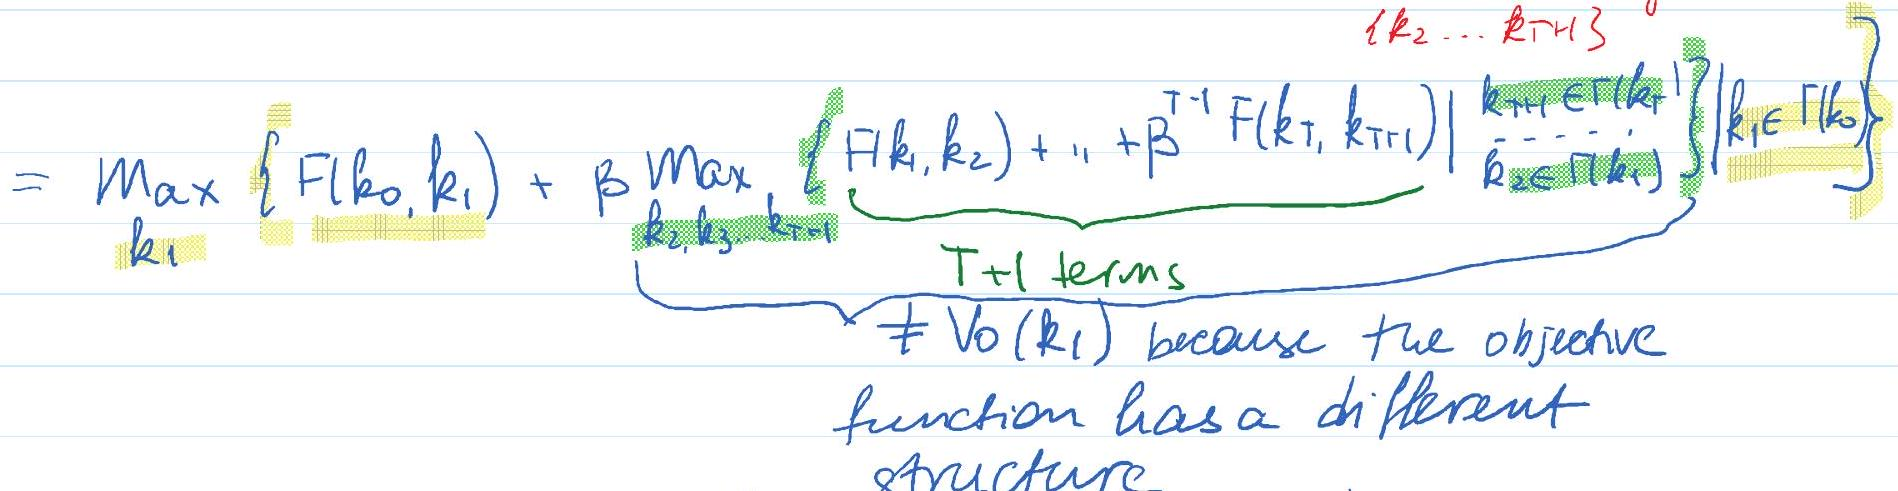
\includegraphics[max width=\textwidth, alt={}, center]{f4cb1c48-88bb-421e-95a2-79ed08ccdae7-8_491_1898_2105_225}\\
denok it by $V_{1}\left(k_{1}\right)$

$$
\begin{aligned}
\Rightarrow V_{0}\left(k_{0}\right) & =\max _{k_{1} \in \Gamma\left(k_{0}\right)}\left\{F\left(k_{0}, k_{1}\right)+\beta V_{1}\left(k_{1}\right)\right\} \\
& \begin{aligned}
V_{t}(k) & =\max _{k^{\prime} \in \Gamma(k)}\left\{F\left(k, k^{\prime}\right)+\beta V_{t+1}\left(k^{\prime}\right)\right\}, t=0 \ldots r-1 \\
\text { at } T: k^{\prime} & =0 \Rightarrow V_{T}(k)=u(\underbrace{f(k)})
\end{aligned}
\end{aligned}
$$

consume everything\\
⇒ The suquence of $\left\{V_{t}(k)\right\}_{t=0}^{T}$ can be solved for "backwards".


\end{document}